\lstset{
  basicstyle=\ttfamily,
  columns=fullflexible,
  frame=single,
  breaklines=true,
  showlines=true,
  postbreak=\mbox{\textcolor{red}{$\hookrightarrow$}\space},
}

\chapter{Implementasi dan Pengujian}
\label{chap:implementasiDanPengujian}

Bab ini membahas proses implementasi dan proses pengujian fitur kolektor pengumuman.
\section{Implementasi}
Bagian ini membahas implementasi dari perancangan yang telah dilakukan di Bab 4. Implementasi ini dilakukan dengan terlebih dahulu membuat akun Heroku lalu membuat aplikasi \textit{web} baru di Heroku dan melakukan \textit{deploy} ke dalamnya. Aplikasi \textit{web} tersebut diberi nama Shadowtape dan dapat diakses di \url{https://shadowtape.herokuapp.com/}. Setelah itu, \textit{source code} BlueTape dimodifikasi ulang sesuai hasil analisis arsitektur Heroku yang digunakan untuk BlueTape dan di-\textit{deploy} lagi. Selain membuat akun Heroku, peneliti juga perlu membuat akun \textit{email} baru dan akun LINE@ baru. Akun \textit{email} baru menggunakan layanan \textit{email} Gmail dengan alamat \href{mail-to:shadowbluetape@gmail.com}{shadowbluetape@gmail.com}. Akun LINE@ bernama Shadowtape.

\subsection{Lingkungan Pengembangan}
Berikut spesifikasi perangkat keras dan perangkat lunak yang dipakai untuk pengembangan pada skripsi ini:

\textbf{Spesifikasi Perangkat keras}
\begin{itemize}
\item Processor Intel® Celeron(R) CPU 1007U @ 1.50GHz x 2 
\item Graphics Intel® Ivybridge Mobile
\item RAM 8 GB
\item Harddisk 500GB SATA
\end{itemize}

\textbf{Spesifikasi Perangkat lunak}
\begin{itemize}
\item Sistem Operasi Ubuntu 18.04.1 LTS 64-bit
\item Visual Studio Code version 1.31.0
\item apache2 -v
\item PHP 7.2.10 (cli)
\item Composer version 1.7.2
\item pgAdmin4 version 2.1 (Application Mode: Desktop)
\item psql (PostgreSQL) 10.6
\item heroku/7.21.0 linux-x64 node-v11.9.0
\end{itemize}

\subsection{Implementasi Basis Data}
Pada pembangunan fitur kolektor pengumuman, ada dua tabel yang ditambahkan. Kedua tabel tersebut adalah tabel Pengumuman dan tabel PengumumanLineFollowers. Pembuatan tabel menggunakan dua \textit{file migration} terpisah: \textit{file} 20181011103200\_Pengumuman\_Initial.php dan 20190210224400\_PengumumanLineFollowers\_initial.php.

\subsection{Implementasi Kelas}
Pada pembangunan fitur kolektor pengumuman, dibuat kelas-kelas berikut: 
\begin{itemize}
\item Kelas \textit{model} Pengumuman\_model

Pengumuman\_model merupakan kelas yang berisi algoritma yang dibutuhkan oleh fitur kolektor pengumuman.

\item Kelas \textit{model} Pengumuman\_Line\_model

Pengumuman\_model merupakan kelas yang dikhususkan untuk algoritma untuk menghubungkan BlueTape dengan LINE API.

\item Kelas \textit{controller} \textit{Cron}

\textit{Cron} merupakan kelas yang berfungsi untuk menjalankan perintah-perintah yang harus dijalankan pada jadwal tertentu. Pada skripsi ini perintah yang dijadwalkan adalah memeriksa \textit{email}. Pada tahap perancangan, perintah untuk memeriksa \textit{email} dijadwalkan tiap lima belas menit. Pada tahap implementasi, perintah tersebut dijadwalkan lebih jarang karena pemakaian \textit{dyno free} dibatasi. Jadwal baru untuk perintah terebut adalah setiap hari pada pukul 12.00 siang.

\item Kelas \textit{controller} Pengumuman

Pengumuman merupakan kelas yang berfungsi untuk mengatur hubungan antara Pengumuman\_model dan \textit{view} yang ada di \textit{package} Pengumuman.

\item Kelas \textit{controller} PengumumanLine

Pengumuman\_Line merupakan kelas yang berfungsi untuk menerima \textit{webhook} dari Line API.

\end{itemize}

Untuk mendukung kinerja kelas-kelas tersebut, dibuat juga \textit{file}:
\begin{itemize}
\item \textit{File view} main.php.

\textit{File} ini digunakan untuk mengatur tampilan halaman utama Pengumuman.

\item \textit{File view} read.php.

\textit{File} ini digunakan untuk mengatur tampilan halaman saat detail pengumuman ditampilkan.

\item \textit{File config} pengumuman.php.

\textit{File} ini digunakan untuk menyimpan daftar pengirim pengumuman yang terverifikasi.

\item \textit{File migration} 20181011103200\_Pengumuman\_Initial.php 

\textit{File} ini digunakan untuk membuat tabel Pengumuman.

\item \textit{File migration} 20190210224400\_PengumumanLineFollowers\_initial.php.

\textit{File} ini digunakan untuk membuat tabel PengumumanLineFollowers.
\end{itemize}

Selain \textit{file yang telah disebutkan}, ada beberapa \textit{file} yang isinya harus diubah:
\begin{itemize}
\item \textit{file} \textit{config} database.php

Pada \textit{file} ini, informasi yang berkaitan dengan basis data disesuaikan dengan informasi basis data yang dipakai di skripsi ini.

\item \textit{file} \textit{config} modules.php

Pada \textit{file} ini, ditambahkan \textit{modules} Pengumuman pada \textit{config} 'modules'.

\item \textit{file} \textit{config} routes.php

Pada \textit{file} ini ditambahkan \textit{routing} berikut:
\begin{lstlisting}
$route['pengumuman/page-(:num)'] = '/pengumuman/page/$1';
\end{lstlisting}
\end{itemize}

\section{Pengujian}
\subsection{Lingkungan Pengujian}
Berikut spesifikasi yang dipakai untuk pengujian pada skripsi ini:
\begin{itemize}
\item Heroku dengan spesifikasi :

\begin{itemize}
\item \textit{Region}: \textit{United States}
\item \textit{Stack}: heroku-18
\item \textit{Framework}: PHP
\item Ukuran maksimum \textit{slug}: 500 MiB
\item Heroku Git URL: url{https://git.heroku.com/shadowtape.git}
\item \textit{Buildpack:} heroku/php
\item \textit{Domain:} \url{https://shadowtape.herokuapp.com/}
\item \textit{Dyno Type: Free Dynos}
\item \textit{Add-ons} Heroku Postgres dan Heroku Scheduler
\end{itemize}

\item Akun \textit{bot} LINE@ dengan \textit{plan Developer}
\end{itemize}

\subsection{Pengujian Fungsional}
Pengujian fungsional dilakukan dengan metode \textit{black box testing}. Berikut adalah hasil pengujiannya :
\begin{itemize}
  \item Pengujian \textit{Filter Email} Pengumuman

    Pengujian ini bertujuan untuk menguji apakah \textit{filter email} pengumuman berfungsi dengan baik. \textit{Email} yang dikirim di pengujian ini memiliki subjek. Hasil pengujian dapat dilihat di Tabel \ref{table:pengujian-fungsional-filter-email}.

    \begin{center}
      \begin{table}[H]
        \caption{Pengujian Filter \textit{Email} Pengumuman}
        \label{table:pengujian-fungsional-filter-email}
        \begin{tabular}{|p{5cm}|p{5cm}|p{5cm}|}
        \hline
        \centering Aksi	& 	\centering Reaksi yang diharapkan &  \multicolumn{1}{c|}{Reaksi Perangkat Lunak} \\
        \hline
        Mengirimkan \textit{email} dengan \textit{email} yang terdaftar lalu menjalankan \textit{Cron}. & \textit{Email} masuk ke basis data dan pengumuman ditampilkan di menu pengumuman. & Reaksi sesuai dengan yang diharapkan. \textit{Email} masuk ke basis data dan pengumuman dapat dilihat di menu pengumuman. \\
        \hline
        Mengirimkan \textit{email} dengan \textit{email} yang tidak terdaftar lalu menjalankan \textit{Cron}. & \textit{Email} tidak masuk ke basis data. & Reaksi sesuai dengan yang diharapkan. \textit{Email} tidak masuk ke basis data. \\
        \hline
        \end{tabular}
    \end{table}
    \end{center}

  \item Pengujian Mengirim \textit{Email} dengan Isi \textit{Email} yang Variatif

    Pengujian ini bertujuan untuk menguji apakah isi \textit{email} yang ditampilkan sesuai dengan yang diharapkan. Pengujian ini dilakukan dengan mengirimkan beberapa \textit{email} dengan isi yang berbeda melalui salah satu \textit{email} yang terdaftar di BlueTape, yaitu alamat \textit{email} \href{mailto:shadowbluetape@gmail.com}{shadowbluetape@gmail.com}. Hasil pengujian dapat dilihat di Tabel ~\ref{table:pengujian-fungsional-isi-variatif}.

      \begin{longtable}{|p{5cm}|p{5cm}|p{5cm}|}
        \caption{Pengujian Mengirim \textit{Email} dengan Isi \textit{Email} yang Variatif}
        \label{table:pengujian-fungsional-isi-variatif}\\
        \hline
        \centering Aksi	& 	\centering Reaksi yang diharapkan &  \multicolumn{1}{c|}{Reaksi Perangkat Lunak} \\
        \hline
        Mengirimkan \textit{email} tanpa subjek lalu menjalankan \textit{Cron}. & \textit{Email} tidak masuk ke basis data. & Reaksi sesuai dengan yang diharapkan. \textit{Email} tidak masuk ke basis data. \\
        \hline
        Mengirimkan \textit{email} tanpa isi lalu menjalankan \textit{Cron}. & \textit{Email} masuk ke basis data dan pengumuman ditampilkan di menu pengumuman. & Reaksi sesuai dengan yang diharapkan. \textit{Email} masuk ke basis data dan pengumuman dapat dilihat di menu pengumuman. \\
        \hline
        Mengirimkan \textit{email} dengan subjek dan isi lalu menjalankan \textit{Cron}. & \textit{Email} masuk ke basis data dan pengumuman ditampilkan di menu pengumuman. & Reaksi sesuai dengan yang diharapkan. \textit{Email} masuk ke basis data dan pengumuman dapat dilihat di menu pengumuman. \\
        \hline
        Mengirimkan \textit{email} balasan lalu menjalankan \textit{Cron}. & \textit{Email} masuk ke basis data dan pengumuman ditampilkan di menu pengumuman. & Reaksi sesuai dengan yang diharapkan. \textit{Email} masuk ke basis data dan pengumuman dapat dilihat di menu pengumuman. \\
        \hline
        Mengirimkan \textit{email} terusan lalu menjalankan \textit{Cron}. & \textit{Email} masuk ke basis data dan pengumuman ditampilkan di menu pengumuman. & Reaksi sesuai dengan yang diharapkan. \textit{Email} masuk ke basis data dan pengumuman dapat dilihat di menu pengumuman. \\
        \hline
        Mengirimkan \textit{email} dengan lampiran lalu menjalankan \textit{Cron}. & \textit{Email} masuk ke basis data dan pengumuman ditampilkan di menu pengumuman. Di bawah isi pengumuman, ada keterangan "*) Pengumuman ini memiliki lampiran, silahkan memeriksa langsung \textit{email} student Anda untuk mengunduhnya.". & Reaksi sesuai dengan yang diharapkan. \textit{Email} masuk ke basis data dan pengumuman dapat dilihat di menu pengumuman. Di bawah isi pengumuman, keterangan "*) Pengumuman ini memiliki lampiran, silahkan memeriksa langsung \textit{email} student Anda untuk mengunduhnya." berhasil ditampilkan. \\
        \hline
        Mengirimkan \textit{email} yang terdapat sisipan lampiran berupa gambar di isi \textit{email} lalu menjalankan \textit{Cron}. & \textit{Email} masuk ke basis data dan pengumuman ditampilkan di menu pengumuman. Di bawah isi pengumuman, ada keterangan "*) Pengumuman ini memiliki lampiran, silahkan memeriksa langsung \textit{email} student Anda untuk mengunduhnya.". Isi pesan harus masih lengkap walaupun gambar tidak akan berhasil ditampilkan (karena \textit{file} gambar tidak bisa disimpan di server). & Reaksi sesuai dengan yang diharapkan. \textit{Email} masuk ke basis data dan pengumuman dapat dilihat di menu pengumuman. Di bawah isi pengumuman, keterangan "*) Pengumuman ini memiliki lampiran, silahkan memeriksa langsung \textit{email} student Anda untuk mengunduhnya." berhasil ditampilkan. Isi pesan lengkap. Sesuai ekspektasi, gambar tidak bisa ditampilkan. Namun, ada keterangan alt yang berisi nama \textit{file}.\\
        \hline
        Mengirimkan \textit{email} yang isinya memakai berbagai jenis pemformatan yang bisa dilakukan di gmail, emoji yang disediakan gmail, dan sisipan URL. Setelah itu menjalankan \textit{Cron}. & \textit{Email} masuk ke basis data dan pengumuman ditampilkan di menu pengumuman. Isi \textit{email} lengkap. Pemformatan tetap sama. Emoji tidak diharapkan bisa ditampilkan. Sisipan URL dapat ditampilkan dan URL dapat dikunjungi. & Reaksi sesuai dengan yang diharapkan. \textit{Email} masuk ke basis data dan pengumuman dapat dilihat di menu pengumuman. Isi \textit{email} lengkap. Pemformatan tetap sama. Emoji dapat ditampilkan. Beberapa emoji berubah bentuk tapi tetap memiliki bentuk yang sama. Beberapa emoji persis sama dengan yang ada di isi \textit{email} yang asli. Sisipan URL dapat ditampilkan dan URL dapat dikunjungi. \\
        \hline
    \end{longtable}

    \item Pengujian Notifikasi LINE

    Pengujian ini bertujuan untuk menguji apakah notifikasi LINE dapat terkirim ke bot LINE. Tabel \ref{table:pengujian-fungsional-notifikasi-line}.

    \begin{center}
      \begin{table}[H]
        \caption{Pengujian Notifikasi LINE}
        \label{table:pengujian-fungsional-notifikasi-line}
        \begin{tabular}{|p{5cm}|p{5cm}|p{5cm}|}
        \hline
        \centering Aksi	& 	\centering Reaksi yang diharapkan &  \multicolumn{1}{c|}{Reaksi Perangkat Lunak} \\
        \hline
        Follow akun bot. & User Id LINE tercatat di basis data. & Reaksi sesuai dengan yang diharapkan. User Id LINE berhasil tercatat di basis data.\\
        \hline 
        Mengirimkan \textit{email} dengan \textit{email} yang terdaftar lalu menjalankan \textit{Cron}. \textit{Email} harus memiliki subjek. & Setelah \textit{Cron} sukses dijalankan, notifikasi LINE dari akun bot muncul. & Reaksi sesuai dengan yang diharapkan. Notifikasi LINE dari akun bot muncul. \\
        \hline
        Membuka pesan LINE yang masuk. Setelah itu membuka URL yang tercantum di pesan. & URL dapat dibuka. Apabila belum \textit{login} ke BlueTape, pengguna akan diarahkan ke menu \textit{login}. Setelah \textit{login}, pengguna diarahkan kembali ke URL tersebut. & Reaksi sesuai dengan yang diharapkan. URL dapat dibuka. Apabila belum \textit{login} ke BlueTape, pengguna akan diarahkan ke menu \textit{login}. Setelah \textit{login}, pengguna diarahkan kembali ke URL tersebut.  \\
        \hline
        \end{tabular}
    \end{table}
    \end{center}
\end{itemize}


\subsection{Pengujian Eksperimental}
\begin{figure}[H]
	\centering  
	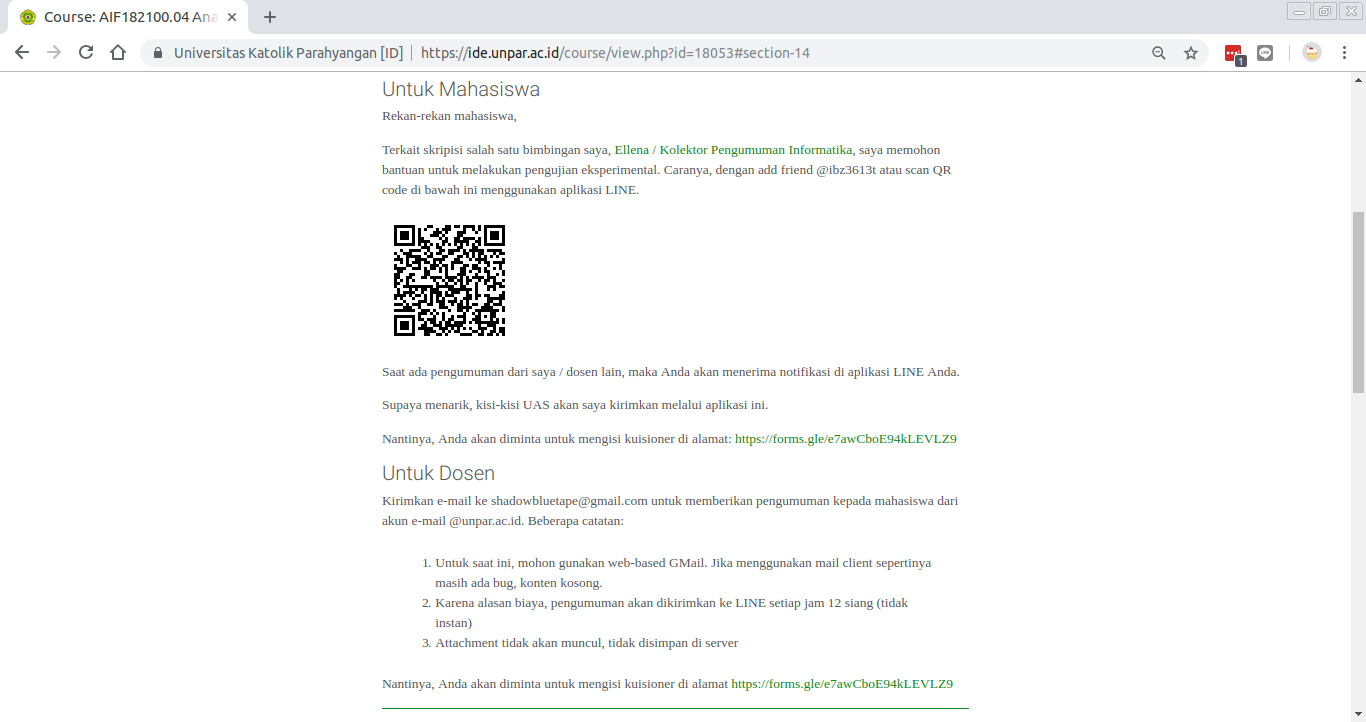
\includegraphics[width=\textwidth]{aif182100-21-27Apr.png}
	\caption[Pengumuman Ujian Eksperimental]{Pengumuman Ujian Eksperimental} 
	\label{fig:aif182100-21-27Apr} 
\end{figure}
Pengujian eksperimental untuk aplikasi ini dilakukan pada mata kuliah AIF182100 (Analisis dan Desain Perangkat Lunak) kelas B dimana dosen kelas tersebut membuat pengumuman kepada mahasiswa untuk melakukan \textit{add friend} dan menunggu pengumuman dari dosen. Pengumuman dapat dilihat pada Gambar~\ref{fig:aif182100-21-27Apr}. Berikut tata cara pengujiannya:
\begin{enumerate}
\item Mahasiswa menambahkan bot Shadowtape dengan mencari id LINE "@ibz3613t" atau memindai kode QR (Gambar~\ref{fig:kode-qr-bot-shadowtape}).

\begin{figure}[H]
	\centering  
	
\includegraphics[scale=0.75]{kode-qr-bot-shadowtape.png}  
	\caption[Kode QR Bot Shadowtape]{Kode QR Bot Shadowtape} 
	\label{fig:kode-qr-bot-shadowtape} 
\end{figure}

\item Dosen mengirimkan \textit{email} berisi pengumuman ke shadowbluetape@gmail.com menggunakan alamat \textit{email} yang terdaftar di BlueTape, yaitu alamat \textit{email} dengan domain unpar.
\item Apabila dosen mengirimkan \textit{email}, maka notifikasi LINE dari akun Shadowtape akan diterima mahasiswa pada pukul 12.00 siang setelah \textit{email} tersebut dikirim.
\item Apabila mahasiswa menerima notifikasi tersebut, mahasiswa akan menerima pesan yang terdapat subjek \textit{email} dan URL di dalamnya. URL tersebut mengarah ke halaman detail pengumuman pada domain \url{http://shadowtape.herokuapp.com/}.
\item Apabila mahasiswa mengklik URL tersebut dan belum \textit{login}, mahasiswa akan diarahkan ke halaman \textit{login} sebelum diarahkan kembali ke URL tersebut.
\item Setelah masa pengujian berakhir, dosen dan mahasiswa mengisi kuesioner pada URL : \url{https://forms.gle/e7awCboE94kLEVLZ9}.
\end{enumerate}

\subsubsection{Pelaksanaan Pengujian}
\begin{figure}[H]
	\centering  
	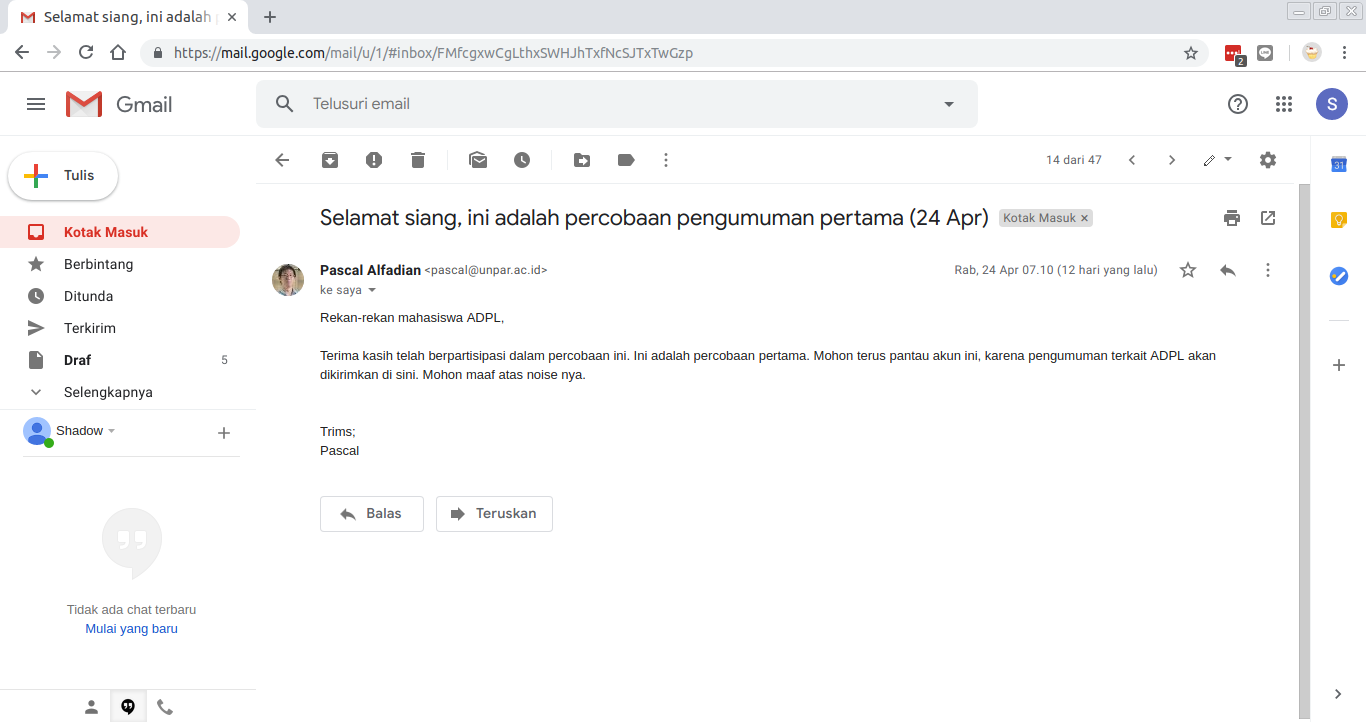
\includegraphics[width=\textwidth]{email-24-april.png}  
	\caption[\textit{Email} pada tanggal 24 April 2019 oleh Bapak Pascal]{\textit{Email} pada tanggal 24 April 2019 oleh Bapak Pascal} 
	\label{fig:email-24Apr} 
\end{figure} 

Pada tanggal 24 April 2019 pukul 07.10, Bapak Pascal Alfadian sebagai dosen mata kuliah AIF182100 (Analisis dan Desain Perangkat Lunak) kelas B mengirimkan \textit{email} ke alamat \textit{email} \href{mailto:shadowbluetape@gmail.com}{shadowbluetape@gmail.com}. Isi \textit{email} dapat dilihat pada Gambar~\ref{fig:email-24Apr}. 

\begin{figure}[H]
	\centering  
	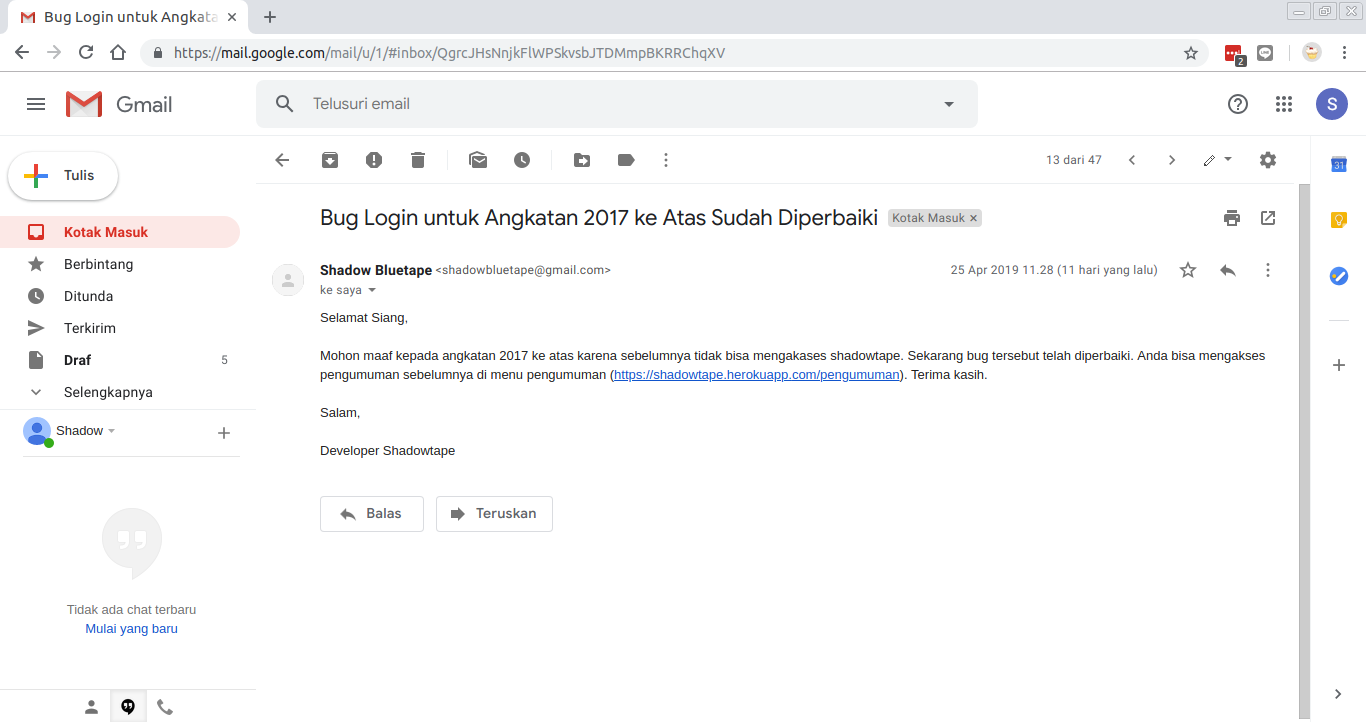
\includegraphics[width=\textwidth]{email-25-april.png}  
	\caption[\textit{Email} pada tanggal 25 April 2019 oleh peneliti]{\textit{Email} pada tanggal 25 April 2019 oleh peneliti} 
	\label{fig:email-25Apr} 
\end{figure}

Pada tanggal 25 April 2019, peneliti menerima laporan bahwa ada masalah \textit{login} untuk angkatan 2017 ke atas. Peneliti menemukan masalah tersebut terjadi karena \textit{repository} skripsi ini ((\url{https://github.com/EllenaAngelica/BlueTape})) tertinggal 4 \textit{commit} dari \textit{repository} asal (\url{https://github.com/ftisunpar/BlueTape}). Peneliti memperbaiki masalah tersebut dengan melakukan \texttt{git pull}. Pada hari tersebut pukul 11.28, peneliti memakai \textit{email} \href{mailto:shadowbluetape@gmail.com}{shadowbluetape@gmail.com} ke alamat \textit{email} ke \href{mailto:shadowbluetape@gmail.com}{shadowbluetape@gmail.com}untuk memberitahu masalah tersebut telah diperbaiki sekaligus melakukan percobaan kedua. Isi \textit{email} dapat dilihat pada Gambar~\ref{fig:email-25Apr}.

\subsubsection{Hasil Pengujian}
\begin{figure}[H]
	\centering  
	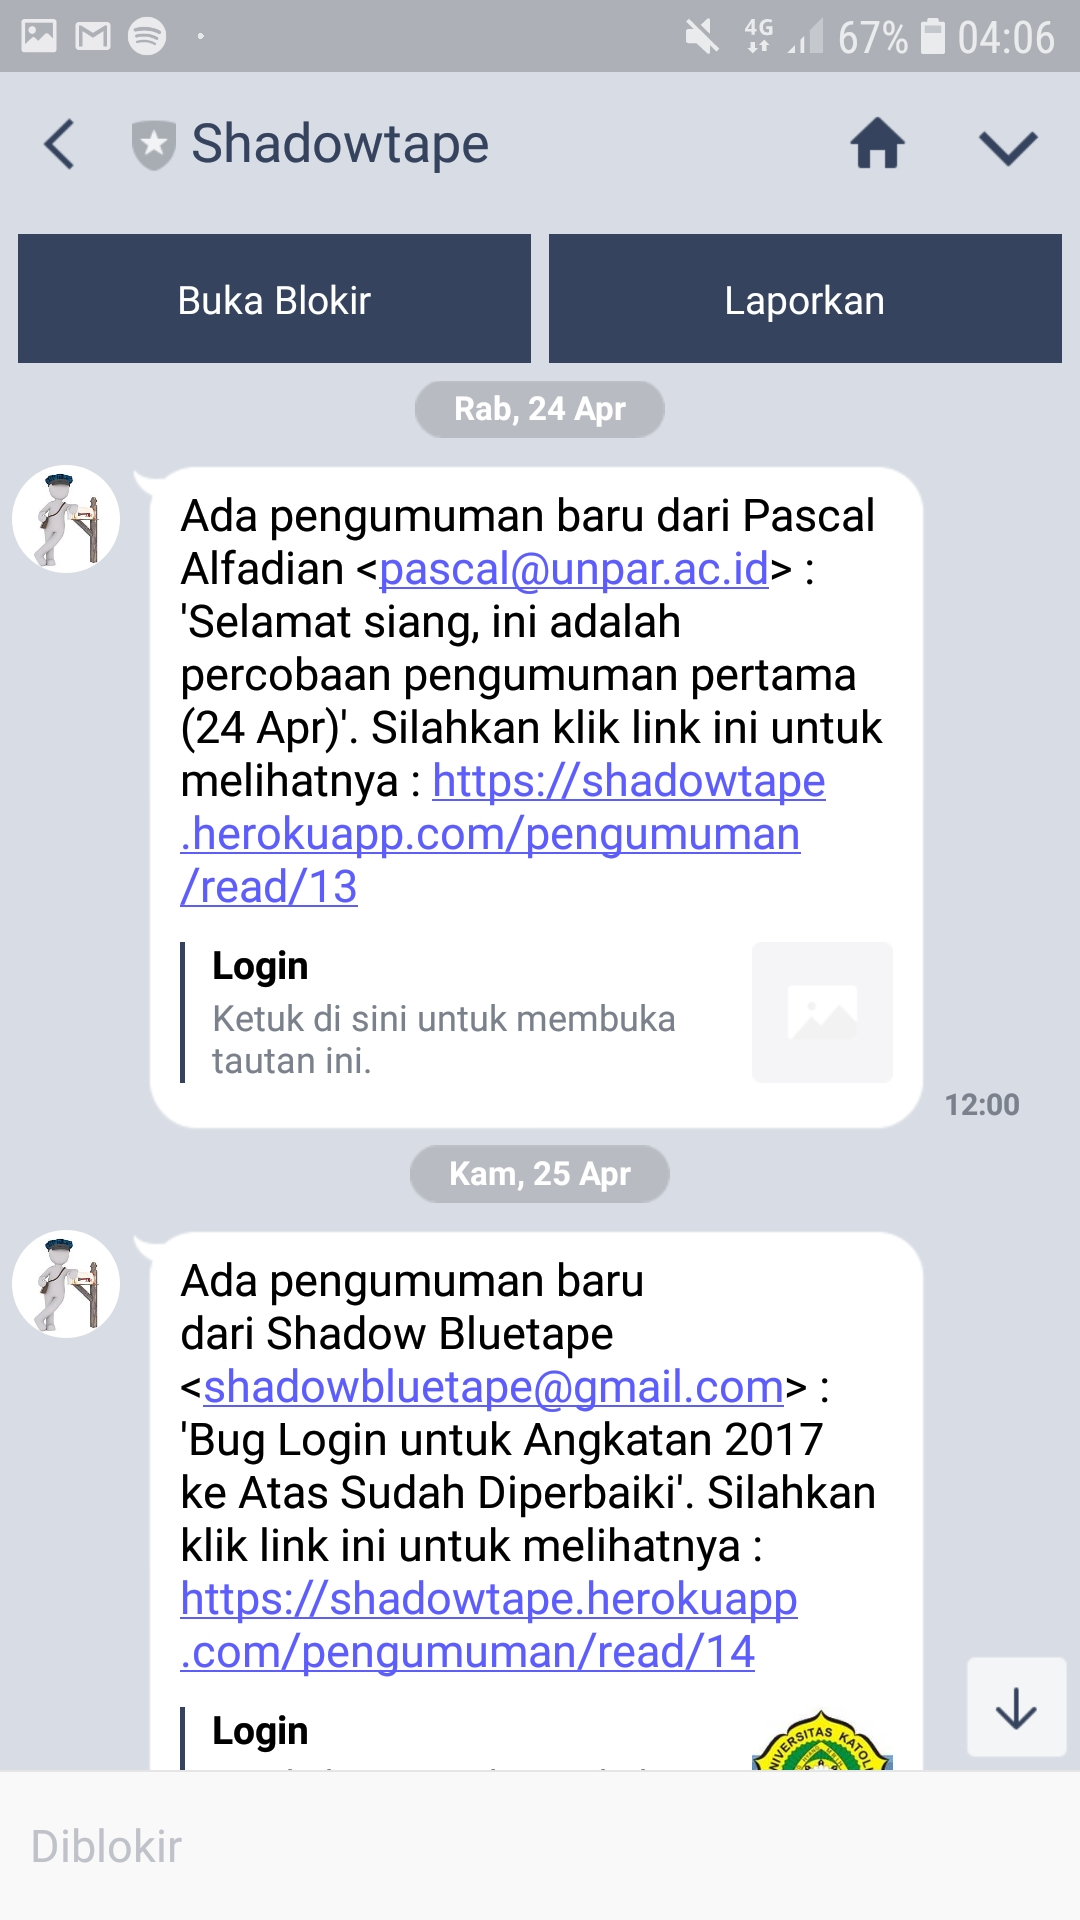
\includegraphics[scale=0.2]{./Hasil-Eksperimental/Screenshot_20190506-040620_LINE.jpg}  
	\caption[Tampilan pesan LINE setelah pengumuman disebar]{Tampilan pesan LINE setelah pengumuman disebar} 
	\label{fig:eks-line} 
\end{figure}
Gambar~\ref{fig:eks-line} menampilkan tampilan pesan LINE yang masuk setelah pengumuman disebar. Karena peneliti tidak sengaja memblokir \textit{bot} Shadowtape dan tidak dapat membuka blokirnya, tampilan pada gambar tersebut memiliki tanda "Diblokir".
\begin{figure}[H]
	\centering  
	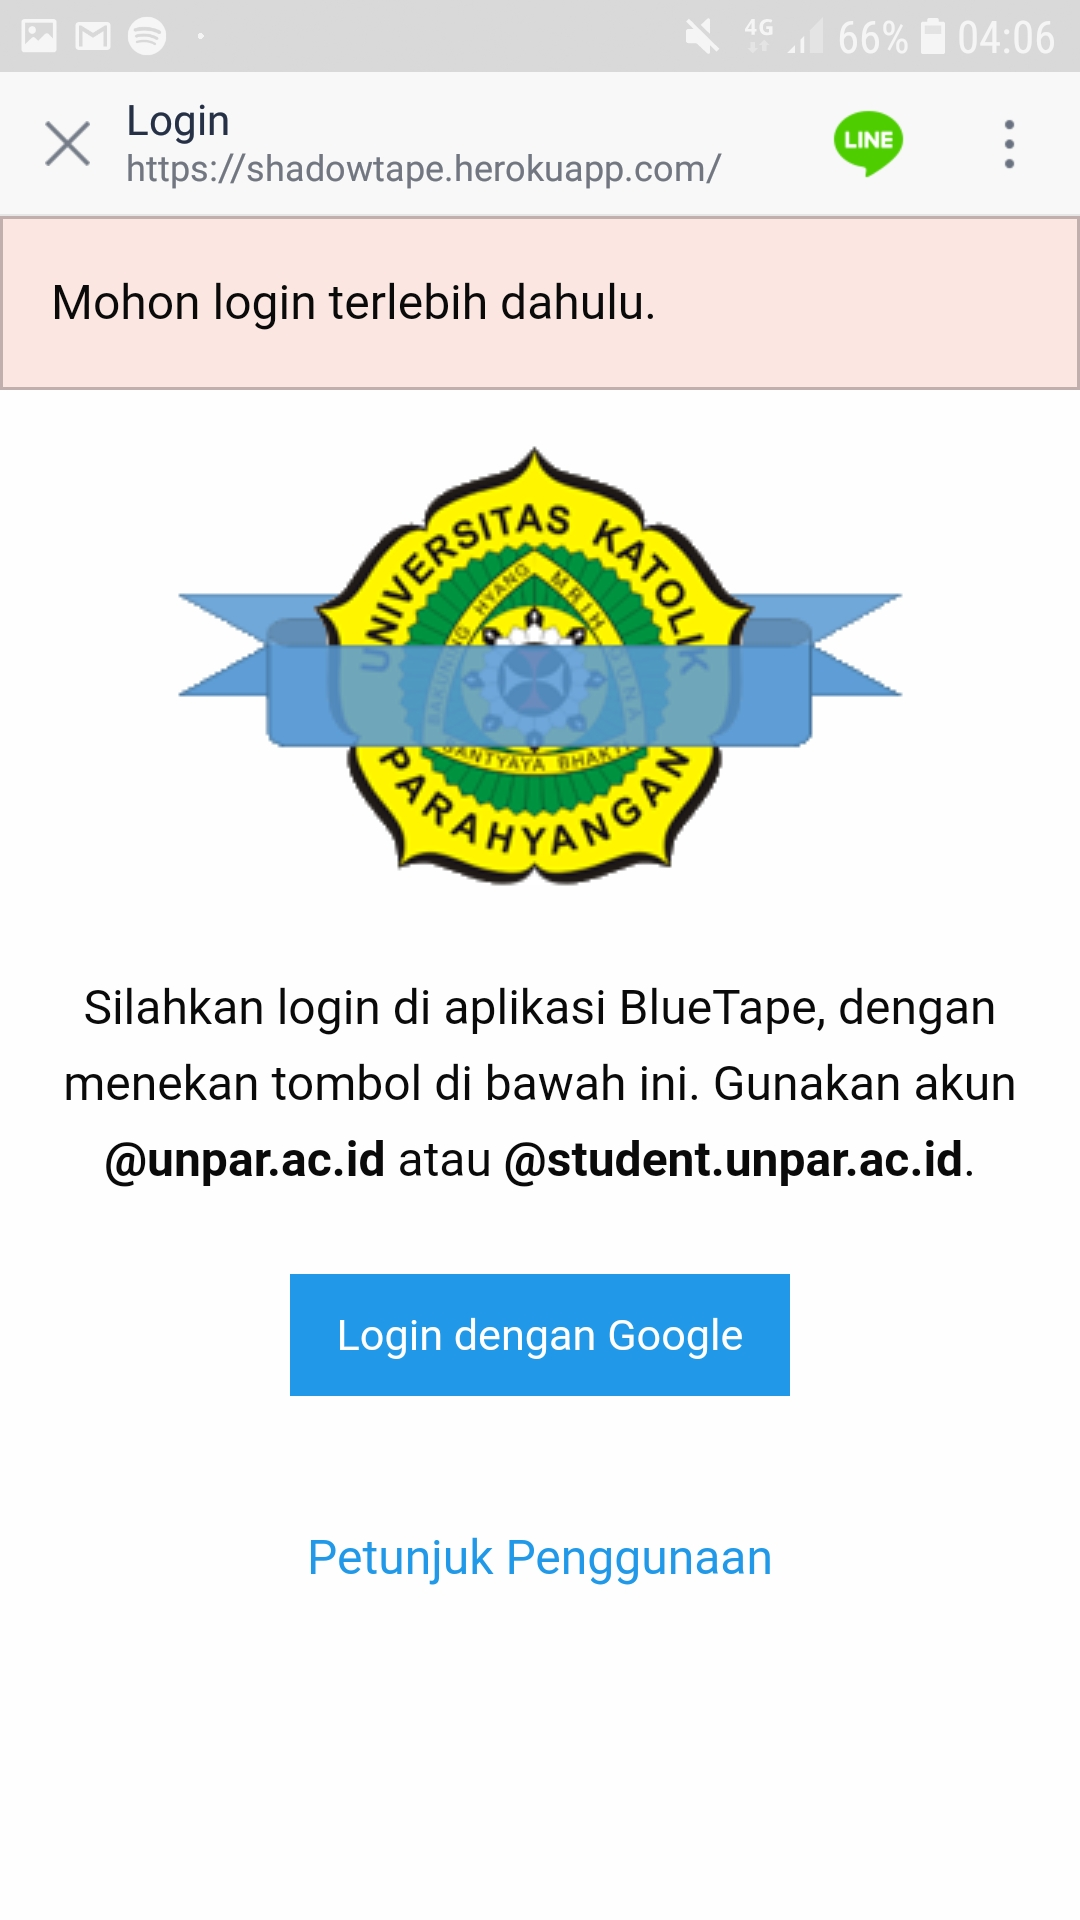
\includegraphics[scale=0.2]{./Hasil-Eksperimental/Screenshot_20190506-040639_LINE.jpg}  
	\caption[Tampilan BlueTape setelah URL dibuka dan pengguna belum \textit{login}]{Tampilan BlueTape setelah URL dibuka dan pengguna belum \textit{login}} 
	\label{fig:eks-belum-login} 
\end{figure}
Gambar~\ref{fig:eks-belum-login} menampilkan tampilan BlueTape setelah URL dibuka dan pengguna belum \textit{login}.
\begin{figure}[H]
	\centering  
	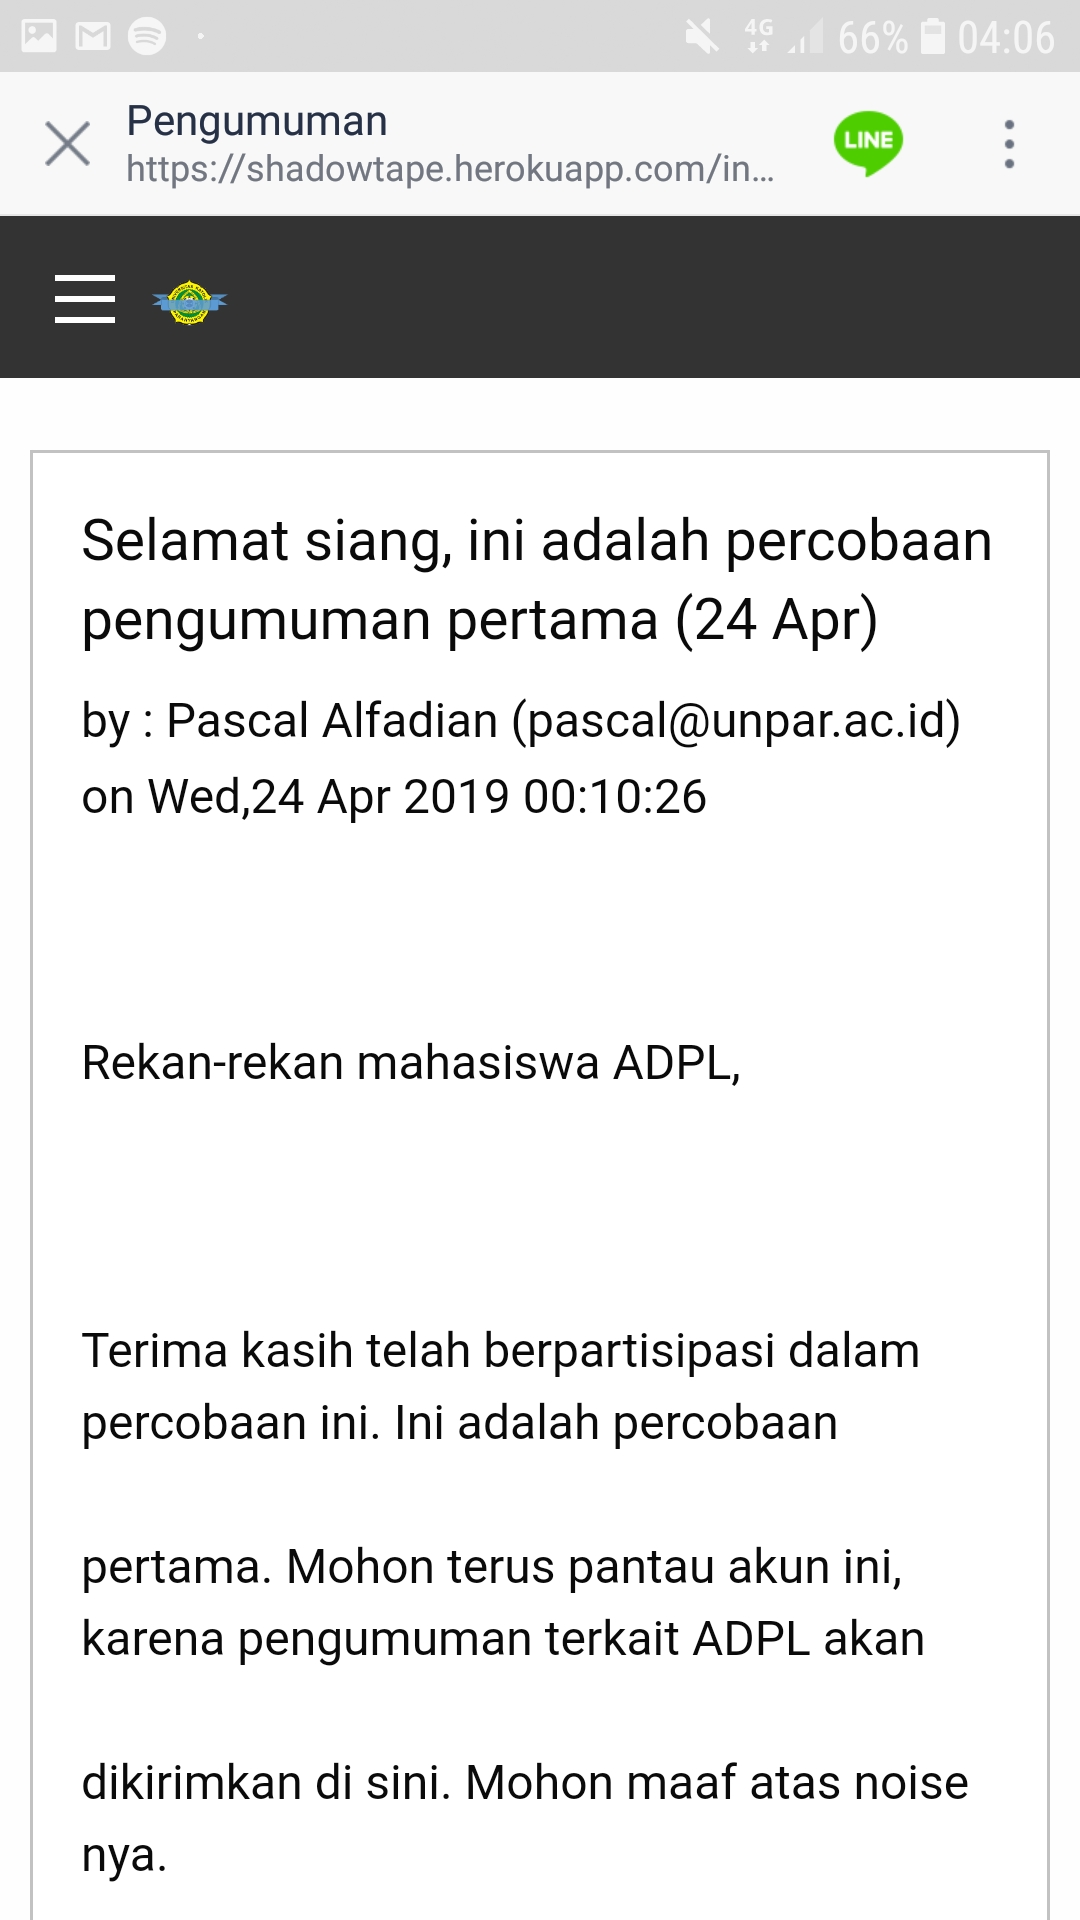
\includegraphics[scale=0.2]{./Hasil-Eksperimental/Screenshot_20190506-040650_LINE.jpg}  
	\caption[Tampilan URL pengumuman yang diumumkan oleh Pak Pascal Alfadian]{Tampilan URL pengumuman yang diumumkan oleh Pak Pascal Alfadian} 
	\label{fig:eks-umum1} 
\end{figure}
Gambar~\ref{fig:eks-umum1} menampilkan tampilan URL pengumuman yang diumumkan oleh Pak Pascal Alfadian.
\begin{figure}[H]
	\centering  
	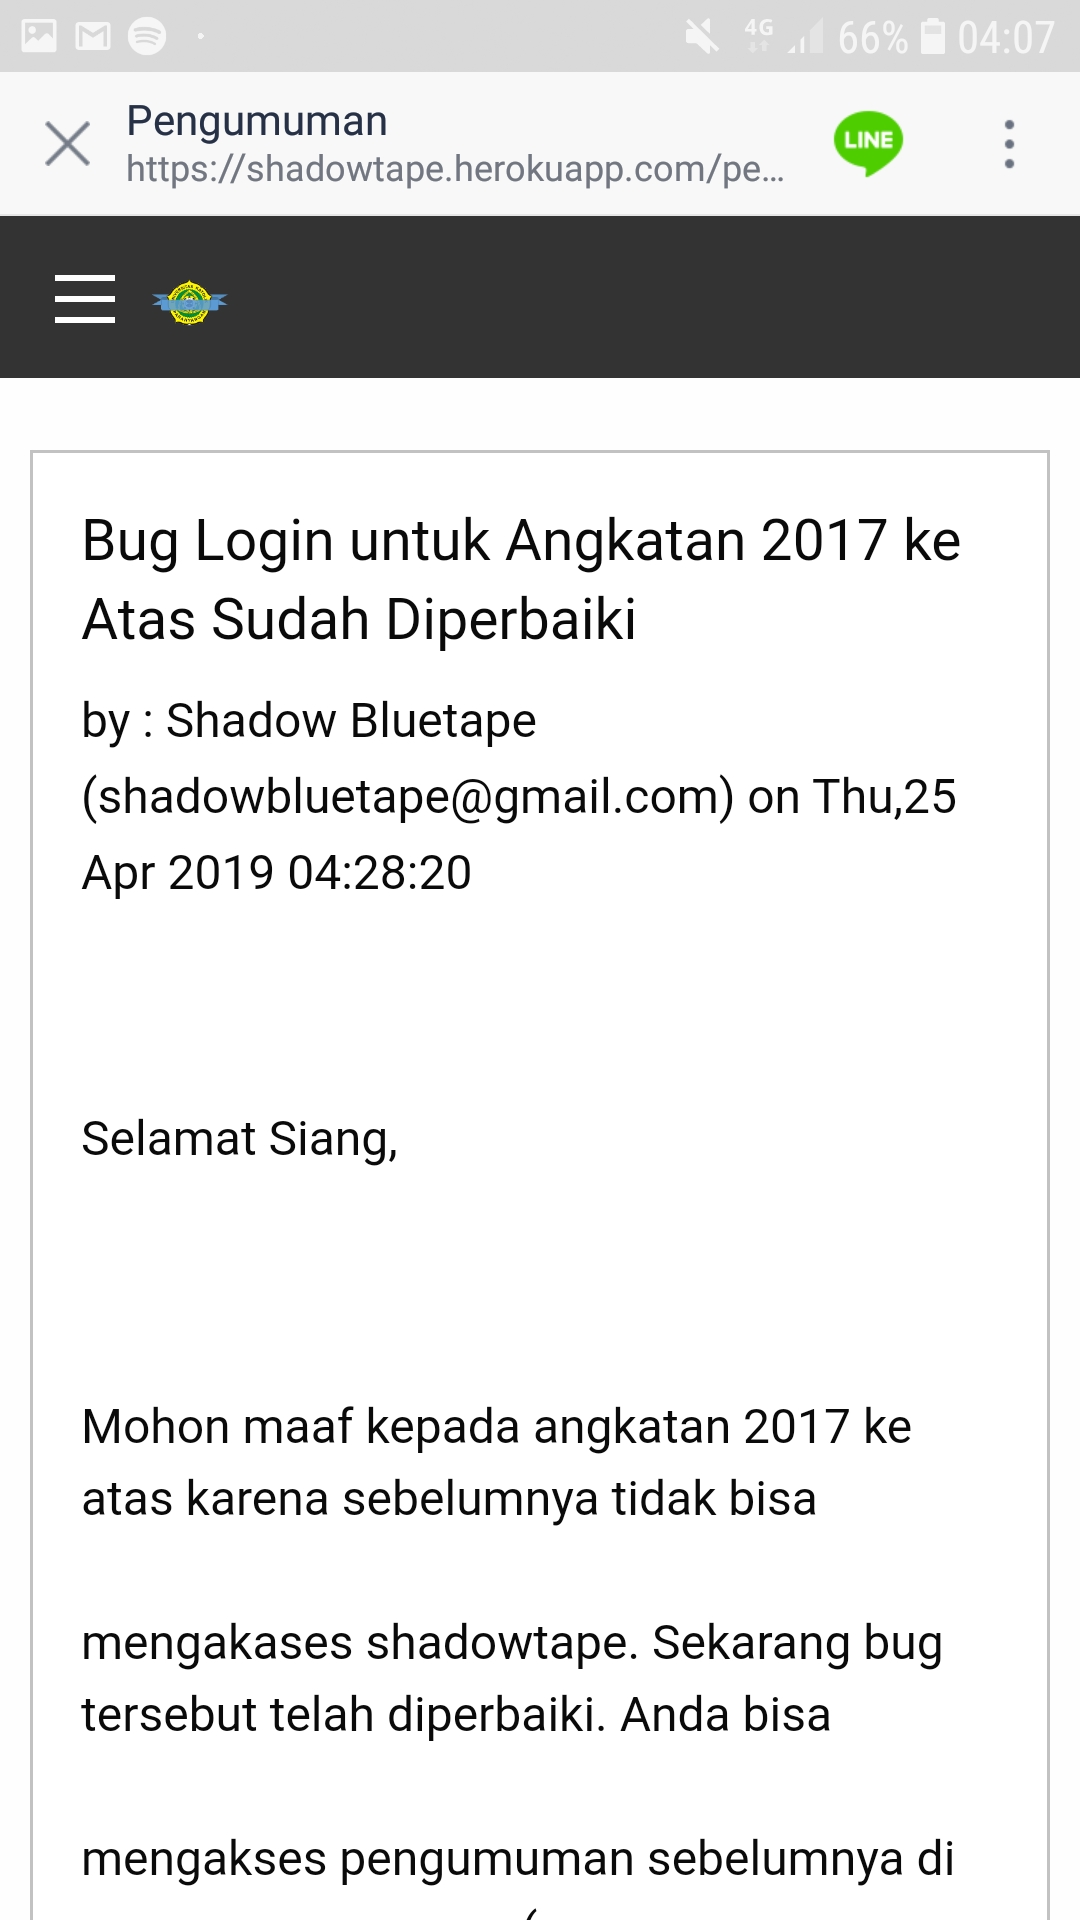
\includegraphics[scale=0.2]{./Hasil-Eksperimental/Screenshot_20190506-040709_LINE.jpg}  
	\caption[Tampilan URL pengumuman yang diumumkan oleh peneliti]{Tampilan URL pengumuman yang diumumkan oleh peneliti} 
	\label{fig:eks-umum2} 
\end{figure}
Gambar~\ref{fig:eks-umum2} menampilkan tampilan URL pengumuman yang diumumkan oleh peneliti.

\subsubsection{Hasil Kuesioner}

\begin{figure}[H]
	\centering  
	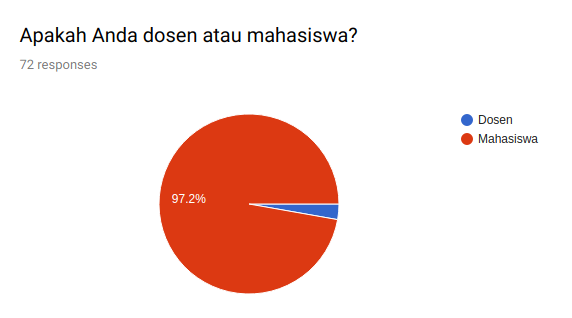
\includegraphics[scale=0.5]{./Survey-Summary/1-Dosen-Mahasiswa.png}
	\caption[Diagram profil responden]{Diagram profil responden} 
	\label{fig:summary-1-Dosen-Mahasiswa} 
\end{figure}

Setelah masa pengujian berakhir, responden yang mengisi kuesioner adalah 72 responden yang terdiri dari 70 mahasiswa dan 2 dosen. Diagram profil responden dapat dilihat pada Gambar~\ref{fig:summary-1-Dosen-Mahasiswa}.

\begin{figure}[H]
	\centering  
	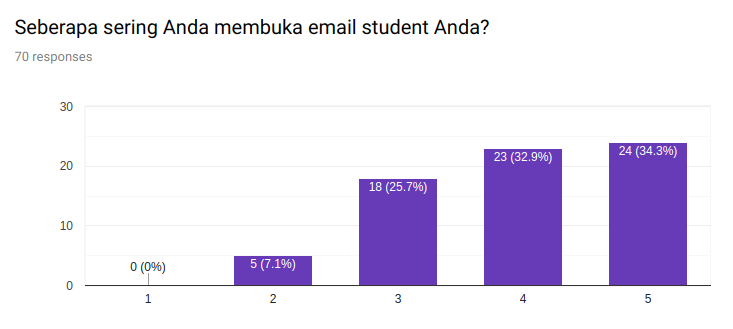
\includegraphics[scale=0.5]{./Survey-Summary/2-Penggunaan-Email.png}
	\caption[Diagram penggunaan \textit{email} di kalangan mahasiswa]{Diagram penggunaan \textit{email} di kalangan mahasiswa} 
	\label{fig:summary-2-Penggunaan-Email} 
\end{figure}

Pada pertanyaan "Seberapa sering Anda membuka \textit{email student} Anda?", mayoritas mahasiswa menjawab 5 (sering sekali). Jumlah mahasiswa yang menjawab 5 (sering sekali) adalah 24 orang. Diagram jawaban untuk pertanyaan ini dapat dilihat pada Gambar~\ref{fig:summary-2-Penggunaan-Email}.

\begin{figure}[H]
	\centering  
	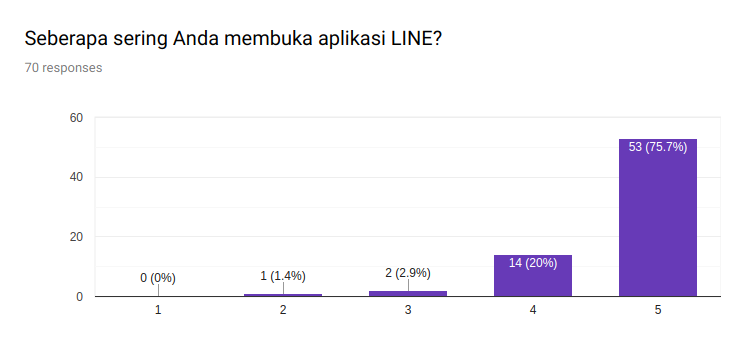
\includegraphics[scale=0.5]{./Survey-Summary/3-Penggunaan-LINE.png}
	\caption[Diagram penggunaan LINE di kalangan mahasiswa]{Diagram penggunaan LINE di kalangan mahasiswa} 
	\label{fig:summary-3-Penggunaan-LINE}
\end{figure}

Pada pertanyaan "Seberapa sering Anda membuka aplikasi LINE?", mayoritas mahasiswa menjawab 5 (sering sekali). Jumlah mahasiswa yang menjawab 5 (sering sekali) adalah 53 orang. Diagram jawaban untuk pertanyaan ini dapat dilihat pada Gambar~\ref{fig:summary-3-Penggunaan-LINE}.

\begin{figure}[H]
	\centering  
	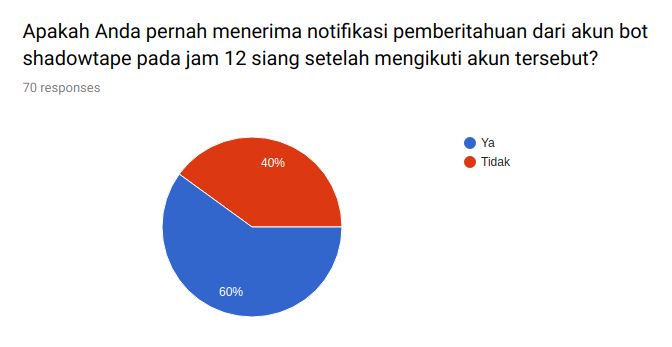
\includegraphics[scale=0.5]{./Survey-Summary/4-Notifikasi-LINE.png}
	\caption[Diagram mahasiswa yang menerima notifikasi LINE]{Diagram mahasiswa yang menerima notifikasi LINE} 
	\label{fig:summary-4-Notifikasi-LINE} 
\end{figure}

Pada pertanyaan "Apakah Anda pernah menerima notifikasi pemberitahuan dari akun bot shadowtape pada jam 12 siang setelah mengikuti akun tersebut?", 42 mahasiswa menjawab "Ya" dan 28 mahasiswa menjawab "Tidak". Diagram jawaban untuk pertanyaan ini dapat dilihat pada Gambar~\ref{fig:summary-4-Notifikasi-LINE}. Mahasiswa yang menjawab "Tidak" belum tentu telah mengikuti \textit{bot} karena jumlah maksimal teman akun LINE@ shadowtape adalah 50 akun. Peneliti memperkirakan jumlah mahasiswa yang tidak mendapatkan notifikasi LINE setelah mengikuti bot LINE tidak lebih dari 8 mahasiswa.

\begin{figure}[H]
	\centering  
	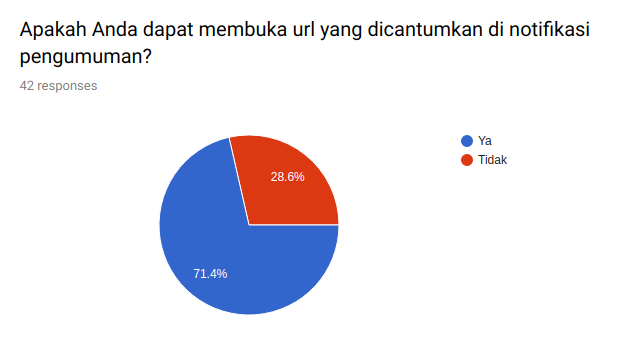
\includegraphics[scale=0.5]{./Survey-Summary/5-Buka-Url.png}
	\caption[Diagram mahasiswa yang dapat membuka URL pengumuman]{Diagram mahasiswa yang dapat membuka URL pengumuman} 
	\label{fig:summary-5-Buka-Url} 
\end{figure}
Pada pertanyaan "Apakah Anda dapat membuka url yang dicantumkan di notifikasi pengumuman?", 30 mahasiswa menjawab "Ya" dan 12 mahasiswa menjawab "Tidak". Diagram jawaban untuk pertanyaan ini dapat dilihat pada Gambar~\ref{fig:summary-5-Buka-Url}. Peneliti menemukan beberapa mahasiswa yang menjawab "Tidak" adalah mahasiswa angkatan 2017 yang masih tidak dapat \textit{login} setelah membaca kolom saran.

\begin{figure}[H]
	\centering  
	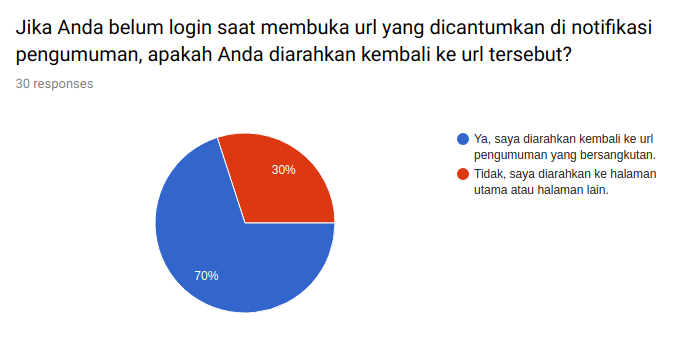
\includegraphics[scale=0.5]{./Survey-Summary/6-Redirect-url.png}
	\caption[Diagram mahasiswa yang diarahkan kembali ke URL pengumuman setelah \textit{login}]{Diagram mahasiswa yang diarahkan kembali ke URL pengumuman setelah \textit{login}} 
	\label{fig:summary-6-Redirect-url} 
\end{figure}

Pada pertanyaan "Jika Anda belum login saat membuka url yang dicantumkan di notifikasi pengumuman, apakah Anda diarahkan kembali ke url tersebut?", 21 mahasiswa menjawab "Ya, saya diarahkan kembali ke url pengumuman yang bersangkutan." dan 9 mahasiswa menjawab "Tidak,  saya diarahkan ke halaman utama atau halaman lain.". Diagram jawaban untuk pertanyaan ini dapat dilihat pada Gambar~\ref{fig:summary-6-Redirect-url}.

\begin{figure}[H]
	\centering  
	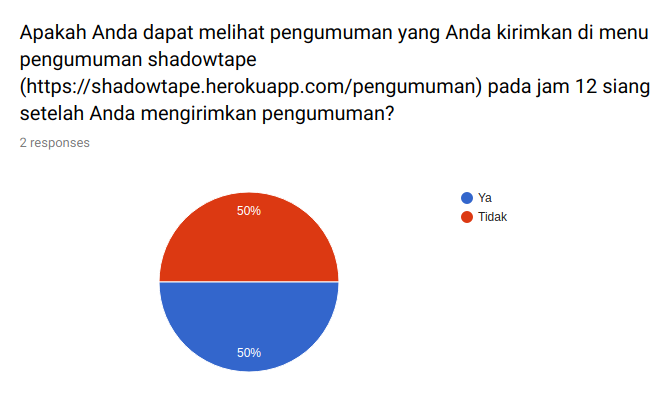
\includegraphics[scale=0.5]{./Survey-Summary/7-Dosen-Lihat-Pengumuman.png}
	\caption[Diagram dosen yang dapat melihat pengumuman yang diumumkannya]{Diagram dosen yang dapat melihat pengumuman yang diumumkannya} 
	\label{fig:summary-7-Dosen-Lihat-Pengumuman} 
\end{figure}

Pada pertanyaan "Apakah Anda dapat melihat pengumuman yang Anda kirimkan di menu pengumuman shadowtape (https://shadowtape.herokuapp.com/pengumuman) pada jam 12 siang setelah Anda mengirimkan pengumuman?", 1 dosen menjawab "Ya" dan 1 dosen menjawab "Tidak". Diagram jawaban untuk pertanyaan ini dapat dilihat pada Gambar~\ref{fig:summary-7-Dosen-Lihat-Pengumuman}. Dosen yang menjawab "Ya" adalah Pak Pascal Alfadian, sedangkan dosen yang menjawab "Tidak" adalah Pak Keenan Adiwijaya Leman. Pak Pascal pernah mengirimkan \textit{email} ke \href{mailto:shadowbluetape@gmail.com}{shadowbluetape@gmail.com} pada tanggal 24 April 2019, sedangkan Pak Keenan tidak pernah.

\begin{figure}[H]
	\centering  
	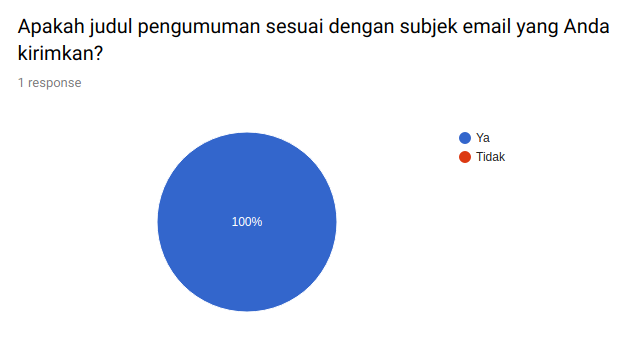
\includegraphics[scale=0.5]{./Survey-Summary/8-Dosen-Judul.png}
	\caption[Diagram dosen yang judul pengumumannya sesuai dengan subjek \textit{email} yang ia kirim]{Diagram dosen yang judul pengumumannya sesuai dengan subjek \textit{email} yang ia kirim} 
	\label{fig:summary-8-Dosen-Judul} 
\end{figure}

Pada pertanyaan "Apakah judul pengumuman sesuai dengan subjek \textit{email} yang Anda kirimkan?", Pak Pascal Alfadian menjawab "Ya". Diagram jawaban untuk pertanyaan ini dapat dilihat pada Gambar~\ref{fig:summary-8-Dosen-Judul}.

\begin{figure}[H]
	\centering  
	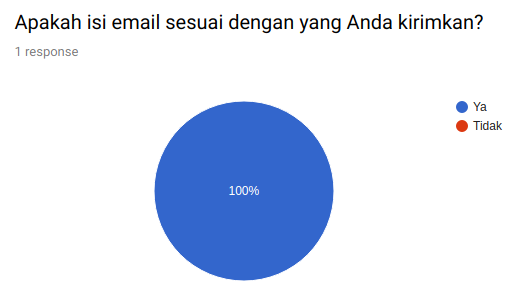
\includegraphics[scale=0.5]{./Survey-Summary/9-Dosen-Isi.png}
	\caption[Diagram dosen yang isi pengumumannya sesuai dengan isi \textit{email} yang ia kirim]{Diagram dosen yang isi  pengumumannya sesuai dengan isi \textit{email} yang ia kirim} 
	\label{fig:summary-9-Dosen-Isi} 
\end{figure}

Pada pertanyaan "Apakah isi \textit{email} sesuai dengan yang Anda kirimkan?", Pak Pascal Alfadian menjawab "Ya". Diagram jawaban untuk pertanyaan ini dapat dilihat pada Gambar~\ref{fig:summary-9-Dosen-Isi}.

\begin{figure}[H]
	\centering  
	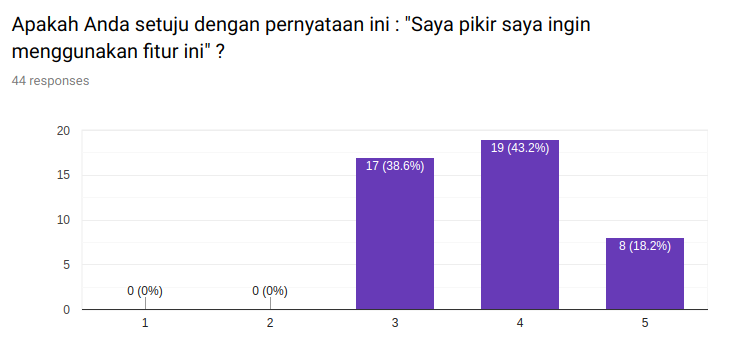
\includegraphics[scale=0.5]{./Survey-Summary/SUS-1.png}
	\caption[Diagram jawaban pertanyaan \textit{System Usability Scale} yang pertama]{Diagram jawaban pertanyaan \textit{System Usability Scale} yang pertama} 
	\label{fig:summary-SUS-1} 
\end{figure}

Pada pertanyaan "Apakah Anda setuju dengan pernyataan ini : "Saya pikir saya ingin menggunakan fitur ini" ?", mayoritas responden menjawab 4 (setuju). Jumlah responden yang menjawab 4 (setuju) adalah 19 orang. Diagram jawaban untuk pertanyaan ini dapat dilihat pada Gambar~\ref{fig:summary-SUS-1}.

\begin{figure}[H]
	\centering  
	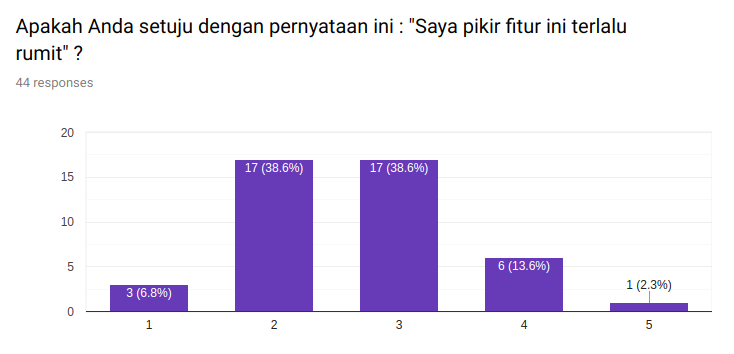
\includegraphics[scale=0.5]{./Survey-Summary/SUS-2.png}
	\caption[Diagram jawaban pertanyaan \textit{System Usability Scale} yang kedua]{Diagram jawaban pertanyaan \textit{System Usability Scale} yang kedua} 
	\label{fig:summary-SUS-2} 
\end{figure}

Pada pertanyaan "Apakah Anda setuju dengan pernyataan ini : "Saya pikir fitur ini terlalu rumit" ?", mayoritas responden menjawab 2 (kurang setuju) dan 3(netral). Jumlah responden yang menjawab 2 (kurang setuju) dan 3(netral) masing-masing 17 orang. Diagram jawaban untuk pertanyaan ini dapat dilihat pada Gambar~\ref{fig:summary-SUS-2}.

\begin{figure}[H]
	\centering  
	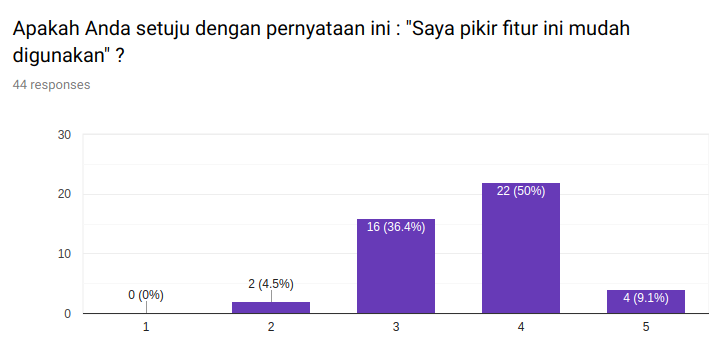
\includegraphics[scale=0.5]{./Survey-Summary/SUS-3.png}
	\caption[Diagram jawaban pertanyaan \textit{System Usability Scale} yang ketiga]{Diagram jawaban pertanyaan \textit{System Usability Scale} yang ketiga} 
	\label{fig:summary-SUS-3} 
\end{figure}

Pada pertanyaan "Apakah Anda setuju dengan pernyataan ini : "Saya pikir fitur ini mudah digunakan" ?", mayoritas responden menjawab 4 (setuju). Jumlah responden yang menjawab 4 (setuju) adalah 22 orang. Diagram jawaban untuk pertanyaan ini dapat dilihat pada Gambar~\ref{fig:summary-SUS-3}.

\begin{figure}[H]
	\centering  
	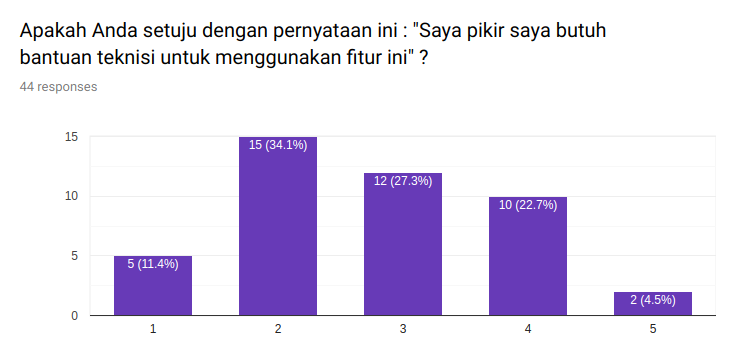
\includegraphics[scale=0.5]{./Survey-Summary/SUS-4.png}
	\caption[Diagram jawaban pertanyaan \textit{System Usability Scale} yang keempat]{Diagram jawaban pertanyaan \textit{System Usability Scale} yang keempat} 
	\label{fig:summary-SUS-4} 
\end{figure}

Pada pertanyaan "Apakah Anda setuju dengan pernyataan ini : "Saya pikir saya butuh bantuan teknisi untuk menggunakan fitur ini" ?", mayoritas responden menjawab 2 (kurang setuju). Jumlah responden yang menjawab 2 (kurang setuju) adalah 15 orang. Diagram jawaban untuk pertanyaan ini dapat dilihat pada Gambar~\ref{fig:summary-SUS-4}.

\begin{figure}[H]
	\centering  
	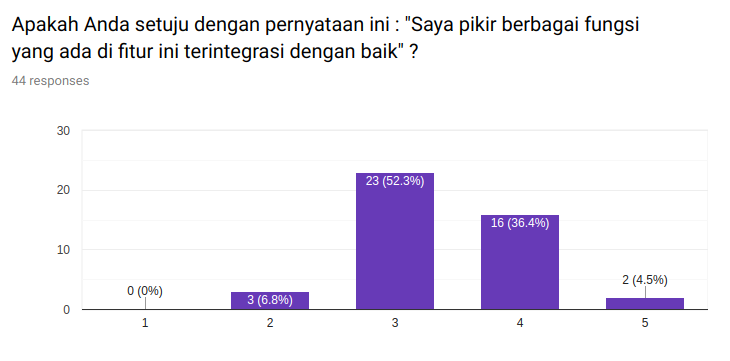
\includegraphics[scale=0.5]{./Survey-Summary/SUS-5.png}
	\caption[Diagram jawaban pertanyaan \textit{System Usability Scale} yang kelima]{Diagram jawaban pertanyaan \textit{System Usability Scale} yang kelima} 
	\label{fig:summary-SUS-5} 
\end{figure}

Pada pertanyaan "Apakah Anda setuju dengan pernyataan ini : "Saya pikir berbagai fungsi yang ada di fitur ini terintegrasi dengan baik" ?", mayoritas responden menjawab 3 (netral). Jumlah responden yang menjawab 3 (netral) adalah 23 orang. Diagram jawaban untuk pertanyaan ini dapat dilihat pada Gambar~\ref{fig:summary-SUS-5}.

\begin{figure}[H]
	\centering  
	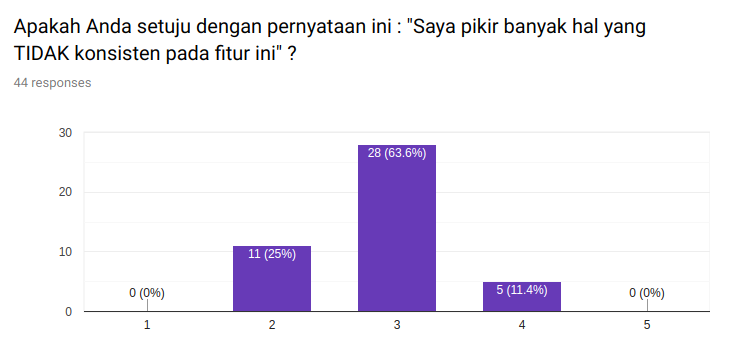
\includegraphics[scale=0.5]{./Survey-Summary/SUS-6.png}
	\caption[Diagram jawaban pertanyaan \textit{System Usability Scale} yang keenam]{Diagram jawaban pertanyaan \textit{System Usability Scale} yang keenam} 
	\label{fig:summary-SUS-6} 
\end{figure}

Pada pertanyaan "Apakah Anda setuju dengan pernyataan ini : "Saya pikir banyak hal yang TIDAK konsisten pada fitur ini" ?", mayoritas responden menjawab 3 (netral). Jumlah responden yang menjawab 3 (netral) adalah 28 orang. Diagram jawaban untuk pertanyaan ini dapat dilihat pada Gambar~\ref{fig:summary-SUS-6}.

\begin{figure}[H]
	\centering  
	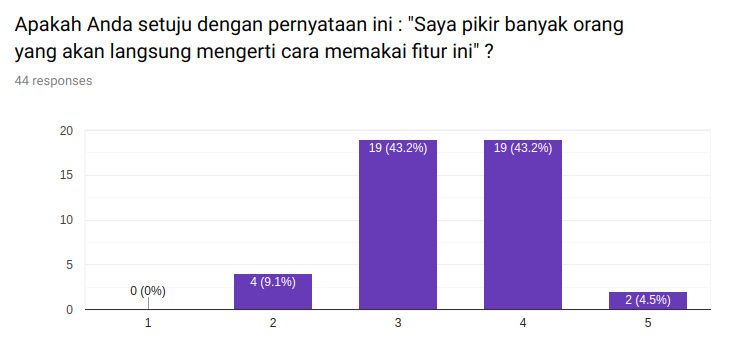
\includegraphics[scale=0.5]{./Survey-Summary/SUS-7.png}
	\caption[Diagram jawaban pertanyaan \textit{System Usability Scale} yang ketujuh]{Diagram jawaban pertanyaan \textit{System Usability Scale} yang ketujuh} 
	\label{fig:summary-SUS-7} 
\end{figure}

Pada pertanyaan "Apakah Anda setuju dengan pernyataan ini : "Saya pikir banyak orang yang akan langsung mengerti cara memakai fitur ini" ?", mayoritas responden menjawab 3 (netral) dan 4 (setuju). Jumlah responden yang menjawab 3 (netral) dan 4 (setuju) masing-masing 19 orang. Diagram jawaban untuk pertanyaan ini dapat dilihat pada Gambar~\ref{fig:summary-SUS-7}.

\begin{figure}[H]
	\centering  
	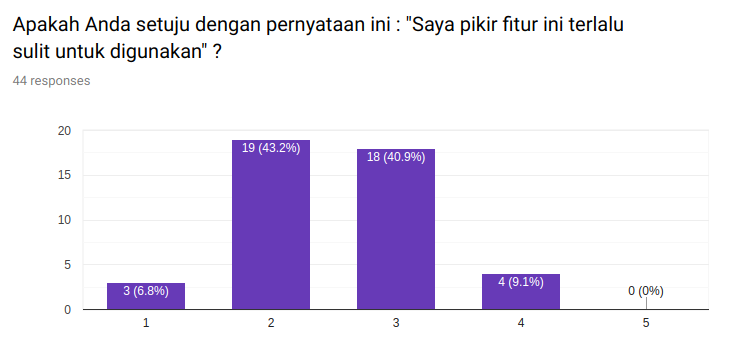
\includegraphics[scale=0.5]{./Survey-Summary/SUS-8.png}
	\caption[Diagram jawaban pertanyaan \textit{System Usability Scale} yang kedelapan]{Diagram jawaban pertanyaan \textit{System Usability Scale} yang kedelapan}
	\label{fig:summary-SUS-8} 
\end{figure}

Pada pertanyaan "Apakah Anda setuju dengan pernyataan ini : "Saya pikir fitur ini terlalu sulit untuk digunakan" ?", mayoritas responden menjawab 2 (kurang setuju). Jumlah responden yang menjawab 2 (kurang setuju) adalah 19 orang. Diagram jawaban untuk pertanyaan ini dapat dilihat pada Gambar~\ref{fig:summary-SUS-8}.

\begin{figure}[H]
	\centering  
	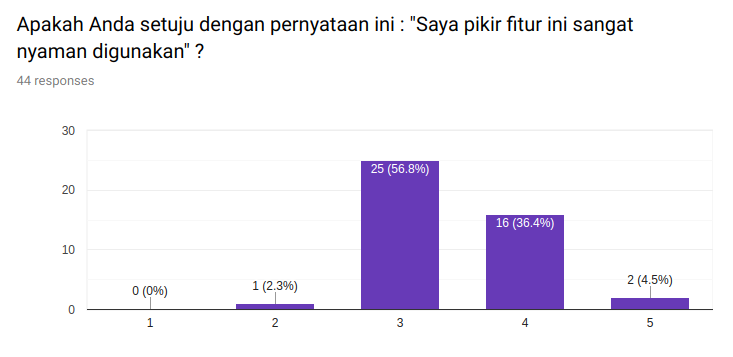
\includegraphics[scale=0.5]{./Survey-Summary/SUS-9.png}
	\caption[Diagram jawaban pertanyaan \textit{System Usability Scale} yang kesembilan]{Diagram jawaban pertanyaan \textit{System Usability Scale} yang kesembilan} 
	\label{fig:summary-SUS-9} 
\end{figure}

Pada pertanyaan "Apakah Anda setuju dengan pernyataan ini : "Saya pikir fitur ini sangat nyaman digunakan" ?", mayoritas responden menjawab 3 (netral). Jumlah responden yang menjawab 3 (netral) adalah 25 orang. Diagram jawaban untuk pertanyaan ini dapat dilihat pada Gambar~\ref{fig:summary-SUS-9}.

\begin{figure}[H]
	\centering  
	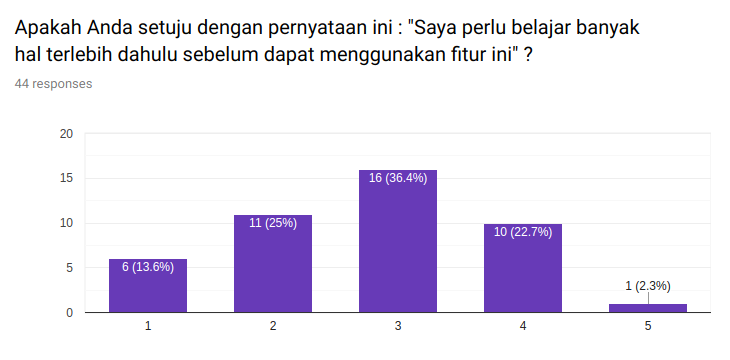
\includegraphics[scale=0.5]{./Survey-Summary/SUS-10.png}
	\caption[Diagram jawaban pertanyaan \textit{System Usability Scale} yang kesepuluh]{Diagram jawaban pertanyaan \textit{System Usability Scale} yang kesepuluh}
	\label{fig:summary-SUS-10} 
\end{figure}

Pada pertanyaan "Apakah Anda setuju dengan pernyataan ini : "Saya perlu belajar banyak hal terlebih dahulu sebelum dapat menggunakan fitur ini" ?", mayoritas responden menjawab 3 (netral). Jumlah responden yang menjawab 3 (netral) adalah 16 orang. Diagram jawaban untuk pertanyaan ini dapat dilihat pada Gambar~\ref{fig:summary-SUS-10}.

\begin{figure}[H]
	\centering  
	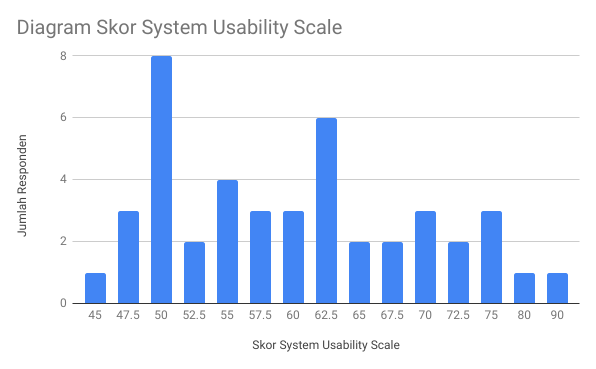
\includegraphics[scale=0.5]{./Survey-Summary/Diagram-Skor-SUS.png}
	\caption[Diagram Skor System Usability Scale]{Diagram Skor System Usability Scale} 
	\label{fig:summary-Diagram-Skor-SUS} 
\end{figure}

Setelah menghitung skor \textit{System Usability Scale} seluruh responden yang menjawab pertanyaan \textit{System Usability Scale}, peneliti mendapatkan rata-ratanya adalah 60,34. Angka tersebut menunjukkan bahwa usabilitas fitur kolektor pengumuman termasuk kelompok rata-rata. Diagram skor \textit{System Usability Scale} dapat dilihat pada Gambar~\ref{fig:summary-Diagram-Skor-SUS}. 

Dari kolom saran, peneliti mendapatkan beberapa saran. Tabel~\ref{table:saran} menampilkan saran yang didapatkan peneliti.

\begin{center}
	\begin{table}[H]
	\caption{Tabel saran}
	\label{table:saran}
	\begin{tabular}{|c|p{11cm}|}
	\hline
  Alamat email	& Saran\\
  \hline
  keenan.leman@unpar.ac.id	& Tidak bisa "add friend" karena akun telah mencapai batas banyak teman.\\
  \hline
  7316027@student.unpar.ac.id	& Lebih diperbagus tampilannya sehingga menarik user untuk menggunakannya\\
  \hline
  7314028@student.unpar.ac.id	& Good Job!\\
  \hline
  2017730022@student.unpar.ac.id	& terdapat beberapa error dalam login, dimana email saya (@student.unpar) tidak memiliki akses\\
  \hline
  2017730047@student.unpar.ac.id	& memperbaiki url login yang dikirimkan di shadowtape\\
  \hline
  2017730011@student.unpar.ac.id	& saran saya, usahakan tidak menggunakan aplikasi luar lain seperti LINE. dikarenakan tidak semua orang menggunakan line\\
  \hline
  2017730037@student.unpar.ac.id	& Link yang dibuka langsung dari line tidak memiliki hak akses\\
  \hline
  2017730008@student.unpar.ac.id	& Fitur ini bagus, memudahkan mahasiswa dalam menerima notifikasi email. Namun, waktunya sebaiknya tidak hanya pada jam 12 siang karena waktu tersebut adalah saat orang-orang makan siang yang mungkin saja sedang tidak membuka gadget/aplikasi Line pada khususnya.\\
  \hline
  2017730044@student.unpar.ac.id	& Log in masih tidak dapat dilakukan, terdapat pernyataan bahwa "alamat email" tidak memiliki hak akses ke pengumuman. Contohnya email yang saya gunakan "2017730044@student.unpar.ac.id tidak memiliki hak akses ke pengumuman"\\
  \hline
  7316025@student.unpar.ac.id	& "Lebih user friendly
"\\
  \hline
	\end{tabular}
	\end{table}
\end{center}

Setelah masa pengujian eksperimental selesai, peneliti menemukan bahwa layanan LINE@ akan diberhentikan. Saat pengujian eksperimental selesai dilaksanakan, pengguna LINE tidak bisa membuat akun LINE@ baru. Sebagai ganti LINE@, LINE membuat layanan baru tapi serupa bernama LINE Official Account. Akun LINE@ yang sudah ada akan diubah menjadi akun LINE Official Account pada bulan Juni 2019.

Perbedaan kedua layanan tersebut terletak pada metode penjualan mereka. LINE@ meminta bayaran apabila pemilik akun LINE@ ingin menambah banyak akun LINE yang dapat menambahkannya sebagai teman, tapi banyak pesan yang dapat dikirim tidak dibatasi. LINE Official Account meminta bayaran apabila pemilik akun LINE Official Account ingin menambah pesan yang dapat ia kirim, tapi jumlah akun yang dapat menambahkannya sebagai teman tidak dibatasi.